%% quizas mover a otro chapter

\chapter{Optimizaciones software}

\section{Optimización mediante distribuciones Bernoulli}

Awano \emph{et al.} \cite{bnn_clt_approx} propusieron muestrear distribuciones Bernoulli en vez de distribuciones gaussianas para aumentar la eficiencia del algoritmo. Los parámetros de estas nuevas distribuciones se obtienen mediante una transformación de los parámetros de las distribuciones originales. Se replicó este método mediante software pero los resultados obtenidos no fueron lo suficientemente buenos en ninguno de los modelos. 

Para el conjunto de datos de píxeles hiperespectrales KSC el modelo optimizado no degradaba la precisión pero en la Figura \ref{fig:bernoulli} se muestra un ejemplo de como las métricas de incertidumbre son alteradas.

\begin{figure}[h]
     \centering
     \begin{subfigure}[b]{0.46\textwidth}
         \centering
         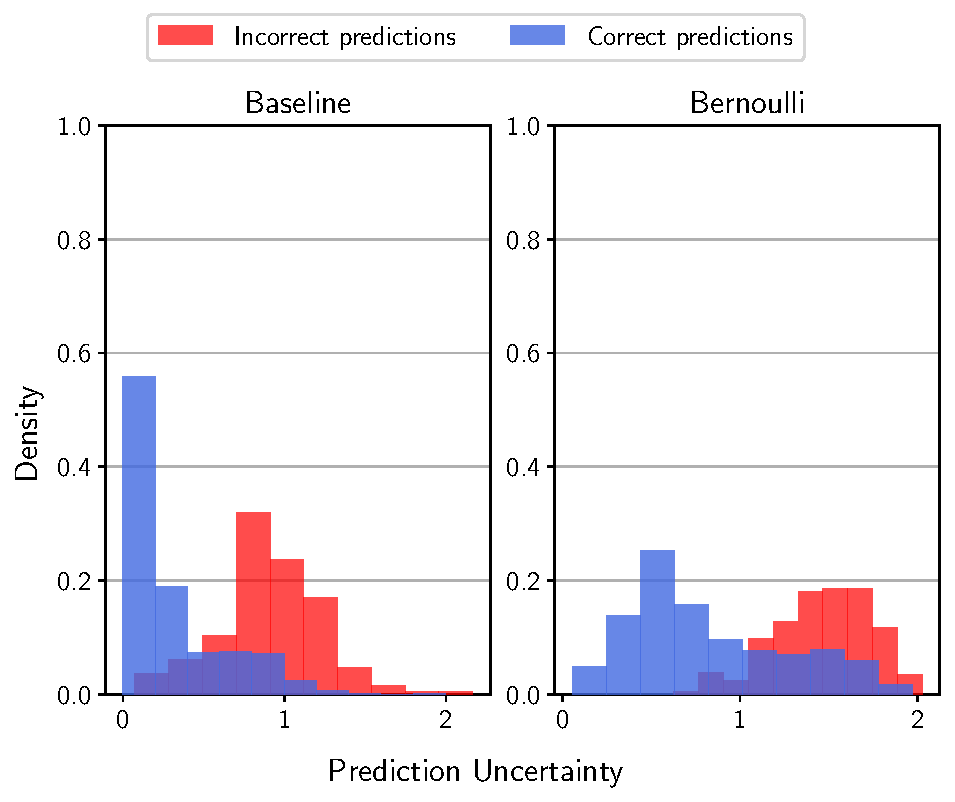
\includegraphics[width=\textwidth]{root/Imagenes/opt_software/bernoulli_hist.pdf}
         \caption{Histogramas de incertidumbre divididos en predicciones correctas (azul) y predicciones incorrectas (rojo).\\ \\}
         \label{fig:bernoulli_hist}
     \end{subfigure}
     \hfill
     \begin{subfigure}[b]{0.51\textwidth}
         \centering
         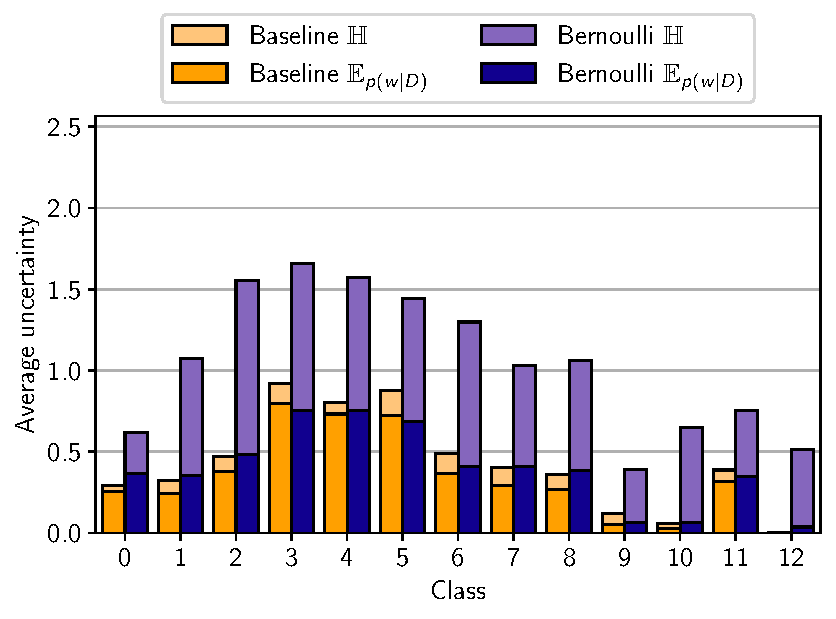
\includegraphics[width=\textwidth]{root/Imagenes/opt_software/bernoulli_class.pdf}
         \caption{Incertidumbre predictiva ($\mathbb{H}$) y aleatoria ($\mathbb{E}p$) agrupada por clases de los resultados obtenidos con TensorFlow (amarillo) y mediante la optimización basada en distribuciones de Bernoulli (azul).}
         \label{fig:bernoulli_class}
     \end{subfigure}
     \caption{Gráficas de análisis de incertidumbre de las predicciones del conjunto de prueba de píxeles hiperespectrales KSC, optimizados mediante distribuciones de Bernoulli y obtenidos mediante TensorFlow.}
     \label{fig:bernoulli}
\end{figure}

Esta degradación de las métricas hace que este modelo pierda una de las principales ventajas de utilizar una BNN por lo que no tiene sentido utilizarlo.

\section{Optimización mediante distribuciones Uniformes}

Este trabajo partiendo de Awano \emph{et al.} propone un nuevo método que utiliza distribuciones Uniformes en vez de distribuciones Bernoulli. El TCL expone que en condiciones generales la distribución de una suma de variables aleatorias tiende a ser una distribución gaussiana. Las operaciones MAC son una suma de variables aleatorias por lo que según el TCL el resultado seguirá una distribución gaussiana. Una distribución gaussiana se define con 2 parámetros, la media y la desviación típica. Asumiendo que el tipo de distribución resultante es independiente del tipo de distribuciones de los sumandos, solamente se tiene que preservar la esperanza y la varianza de la operación MAC para no alterar los resultados de la BNN. Las Ecuaciones \ref{eq:neuron_expected}  y \ref{eq:neuron_variance} muestran la esperanza y la varianza de una operación MAC.
\begin{equation} \label{eq:neuron_expected}
E\left[ b + \sum_{i=0}^N w_i x_i \right]  = b + \sum_{i=0}^N ( E[w_i] E[x_i] )
\end{equation}
\begin{equation} \label{eq:neuron_variance}
V\left[ b + \sum_{i=0}^N w_i x_i \right] = \sum_{i=0}^N ( V[w_i]V[x_i] + V[w_i]E[x_i]^2 + V[x_i]E[w_i]^2 )
\end{equation}

Se propone utilizar un nuevo peso $w'$ que cumpla $E[w'] = E[w]$ y $V[w'] = V[w]$, de forma que no altere los resultados de la BNN. $w' = bu + a$, siendo $u$ una muestra de una distribución Uniforme $\mathcal{U}(0,1)$ y $a$ y $b$ siendo constantes que se pueden calcular a partir de la media $\mu$ y desviación típica $\sigma$ de los pesos originales utilizando el sistema de ecuaciones mostrado en la Ecuación \ref{eq:a_b_equation}.
\begin{equation}\label{eq:a_b_equation}
\begin{cases}
\mu = \dfrac{b}{2} + a\\ \\
\sigma^2 = \dfrac{b^2}{12}
\end{cases}
\rightarrow\ 
\begin{cases}
a = \mu - \dfrac{b}{2}\\ \\
b = \sigma \sqrt{12}
\end{cases}
\end{equation}

Esta optimización no aumenta el tamaño de los modelos y no necesita muestrear distribuciones gaussianas sino uniformes, cuyo algoritmo de muestreo es mucho mas sencillo. La Tabla \ref{tab:uniform_opt} muestra los resultados de precisión y aceleración (\textit{speedup}) obtenidos con esta optimización para todas las arquitecturas de modelos y conjuntos de datos.

\begin{table}[h]
    \centering
    \caption{Resultados de precisión y \textit{speedup} obtenidos con la optimización desarrollada para todas las arquitectruas de modelos y conjuntos de datos.}
    \label{tab:uniform_opt}
    \begin{tabular}{llrrr}
    \hline
     \multirow{2}{*}{\textbf{Modelo}} & \textbf{Conjunto} & \multicolumn{2}{c}{\textbf{Precisión}} & \multirow{2}{*}{\textbf{Speedup}} \\
     & \multicolumn{1}{c}{\textbf{de datos}} & \multicolumn{1}{l}{\textit{TensorFlow}} & \multicolumn{1}{l}{\textit{Optimizado}} & \\ \hline
    \multirow{5}{*}{HYPER} & BO & 0.9039 & 0.9083 & \multirow{5}{*}{4.95} \\
     & IP & 0.8139 & 0.8131 & \\
     & KSC & 0.9256 & 0.9217 & \\
     & PU & 0.9017 & 0.9017 & \\
     & SV & 0.9257 & 0.9280 & \\ \hline
    \multirow{2}{*}{LENET-5} & MNIST & 0.9836 & 0.8906 & \multirow{2}{*}{5.88} \\
     & CIFAR-10 & 0.6351 & 0.4436 & \\ \hline
    \multirow{2}{*}{B2N2} & MNIST & 0.9872 & 0.0964 & \multirow{2}{*}{4.88} \\
     & CIFAR-10 & 0.7295 & 0.2873 & \\ \hline                  
    \end{tabular}
\end{table}

Esta optimización ofrece muy buenos resultados en el caso de los modelos para clasificación de píxeles hiperespectrales, no afectando negativamente a la precisión de los modelos y obteniendo un \textit{speedup} de 4.95. Por contrario, en las arquitecturas de modelos mas le pérdida de precisión es mayor, en el caso del modelo B2N2 llega a ser completamente inaceptable. En el caso del modelo LENET-5 MNIST la precisión obtenida aun puede considerarse lo suficientemente buena la Figura \ref{fig:bad_uncert} muestra como se han degradado las métricas de incertidumbre del modelo. 

%Esta degradación de las métricas hace que este modelo pierda una de las principales ventajas de utilizar una BNN por lo que no tiene sentido utilizarlo.


\begin{figure}[h]
     \centering
     \begin{subfigure}[b]{0.46\textwidth}
         \centering
         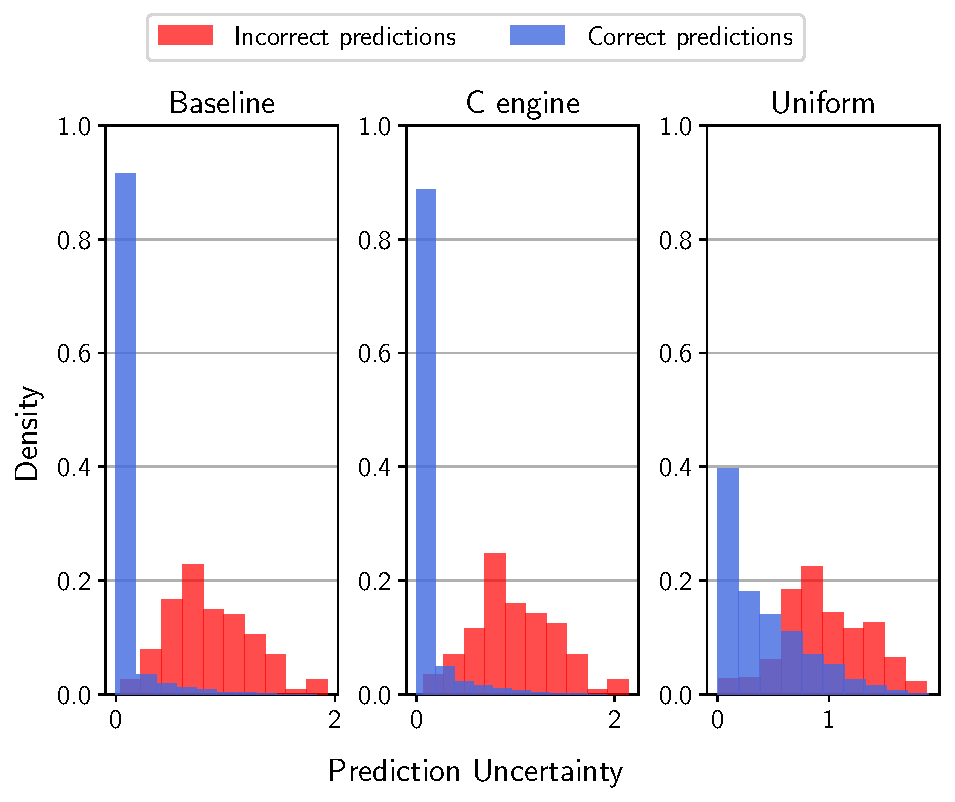
\includegraphics[width=\textwidth]{root/Imagenes/opt_software/hist_uncertainty.pdf}
         \caption{Histogramas de incertidumbre divididos en predicciones correctas (azul) y predicciones incorrectas (rojo).\\}
         \label{fig:bad_uncert_hist}
     \end{subfigure}
     \hfill
     \begin{subfigure}[b]{0.51\textwidth}
         \centering
         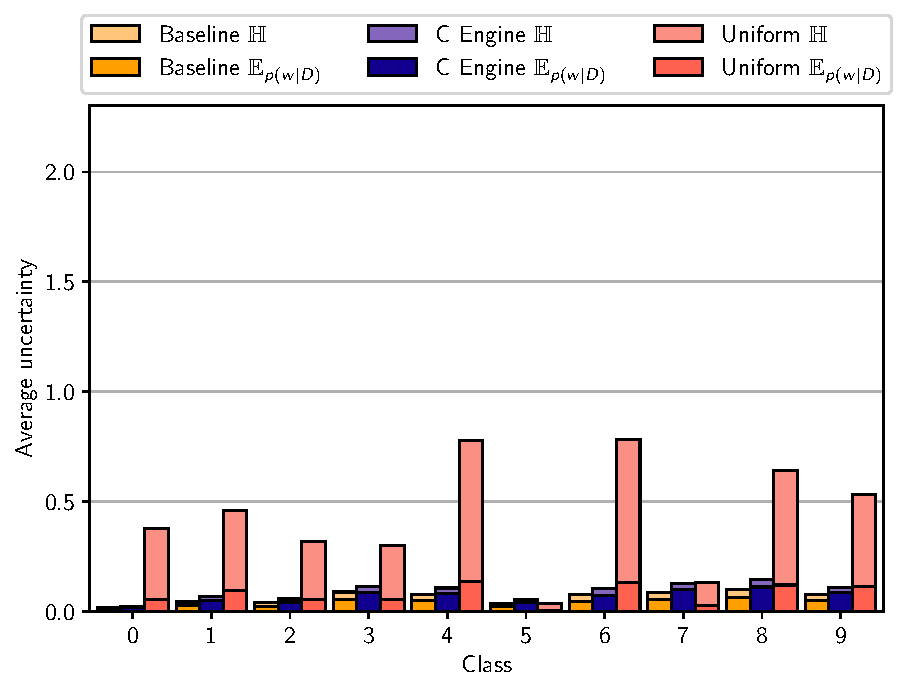
\includegraphics[width=\textwidth]{root/Imagenes/opt_software/class_uncertainty.pdf}
         \caption{Incertidumbre predictiva ($\mathbb{H}$) y aleatoria ($\mathbb{E}p$) agrupada por clases de los resultados obtenidos con TensorFlow (amarillo), el motor de inferencia sin optimización (azul) y con optimización (rojo).}
         \label{fig:bad_uncert_class}
     \end{subfigure}
     \caption{Gráficas de análisis de incertidumbre de los resultados del modelo LENET-5 MNIST optimizado, sin optimizar y obtenidos mediante TensorFlow.}
     \label{fig:bad_uncert}
\end{figure}
